\documentclass[a5paper,11pt,landscape]{article}

\usepackage{main}
\usepackage{array}

\renewcommand{\typedocument}{Document}
\renewcommand{\classe}{5e}
\renewcommand{\titre}{Dipôles électriques}

\begin{document}

\centering
\renewcommand{\arraystretch}{2.2}
\setlength{\tabcolsep}{0.2cm}
\begin{tabular}{|>{\bfseries\centering\arraybackslash}m{2.5cm}
                |>{\centering\arraybackslash}m{4cm}
                |>{\centering\arraybackslash}m{4cm}
                |>{\raggedright\arraybackslash}m{7cm}|}

\hline
\rowcolor{headergrey}
  \textbf{Dipôle} &
  \textbf{Dessin} &
  \textbf{Schéma} &
  \textbf{Description} \\
\hline

Pile
  & 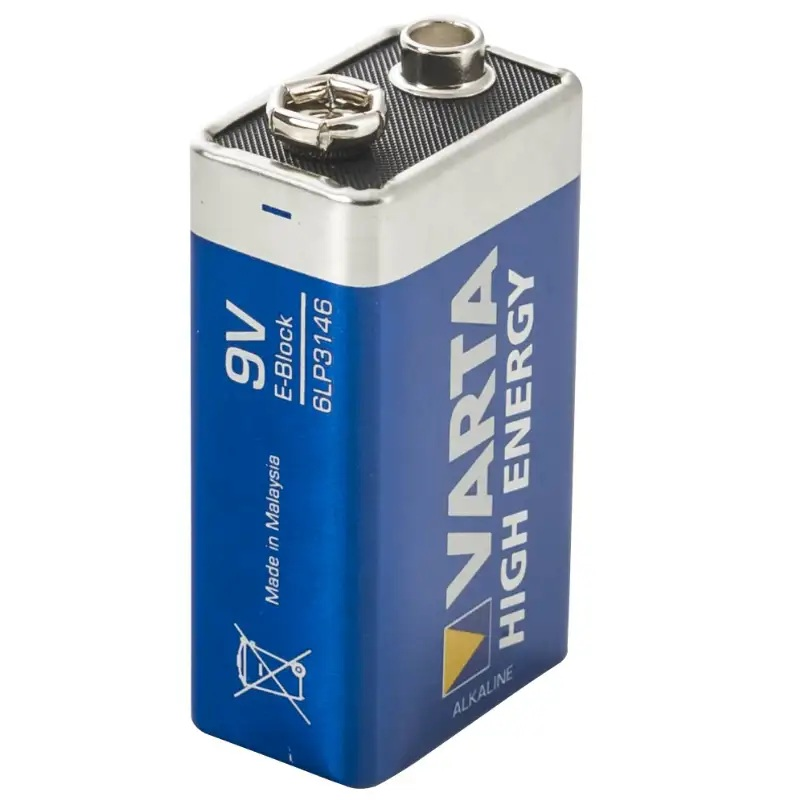
\includegraphics[width=1.35cm]{images/image pile.jpg}
  & % \includegraphics[width=2.5cm]{schema_pile.png}
  & Fournit de l'énergie électrique à partir d'énergie chimique.\\
\hline

Générateur
  & 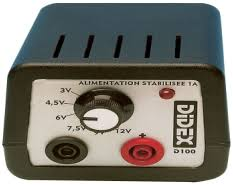
\includegraphics[width=1.35cm]{images/image générateur.jpg}
  & % \includegraphics[width=2.5cm]{schema_generateur.png}
  & Fournit de l'énergie électrique. \\
\hline

Moteur
  & 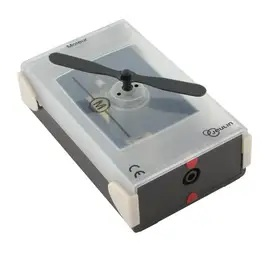
\includegraphics[width=1.35cm]{images/image moteur.jpg}
  & % \includegraphics[width=2.5cm]{schema_moteur.png}
  & Convertit l'énergie électrique en énergie mécanique. \\
\hline

Lampe
  & 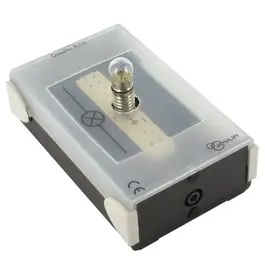
\includegraphics[width=1.35cm]{images/image lampe.jpg}
  & 
  & Convertit l'énergie électrique en énergie lumineuse. \\
\hline

Diode
  & 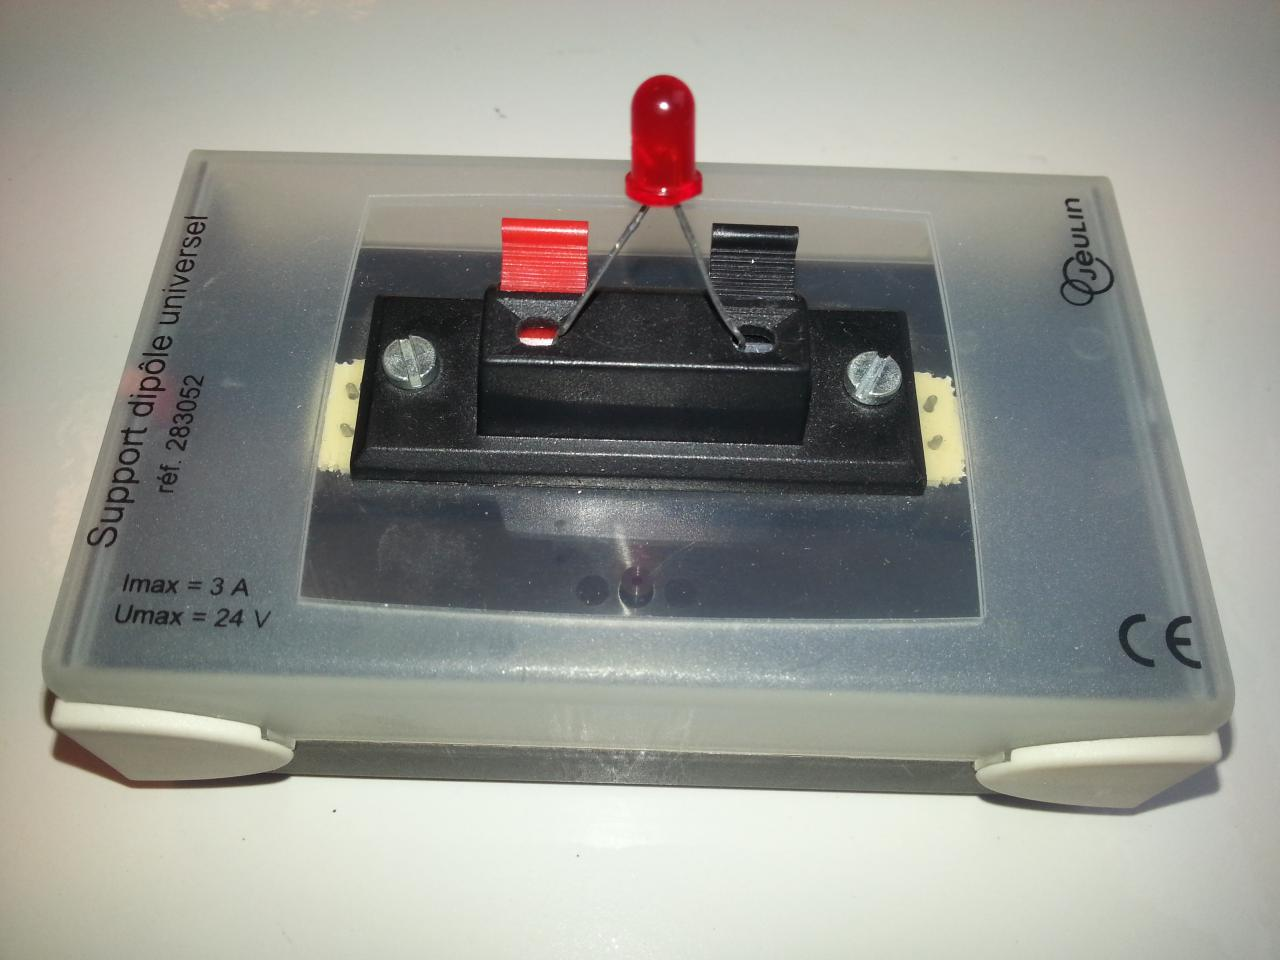
\includegraphics[width=1.35cm]{images/image diode.jpg}
  & % \includegraphics[width=2.5cm]{schema_diode.png}
  & Laisse passer le courant dans un seul sens. \\
\hline

Interrupteur ouvert
  & 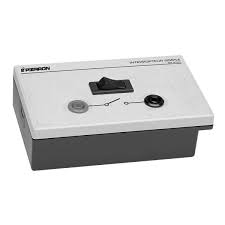
\includegraphics[width=1.35cm]{images/image interrupteur.jpg}
  & % \includegraphics[width=2.5cm]{schema_inter_ouvert.png}
  & Circuit ouvert : le courant ne peut pas circuler. \\
\hline

Interrupteur fermé
  & 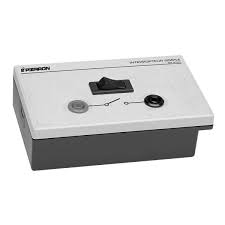
\includegraphics[width=1.35cm]{images/image interrupteur.jpg}
  & % \includegraphics[width=2.5cm]{schema_inter_ferme.png}
  & Circuit fermé : le courant peut circuler. \\
\hline

\end{tabular}

\end{document}